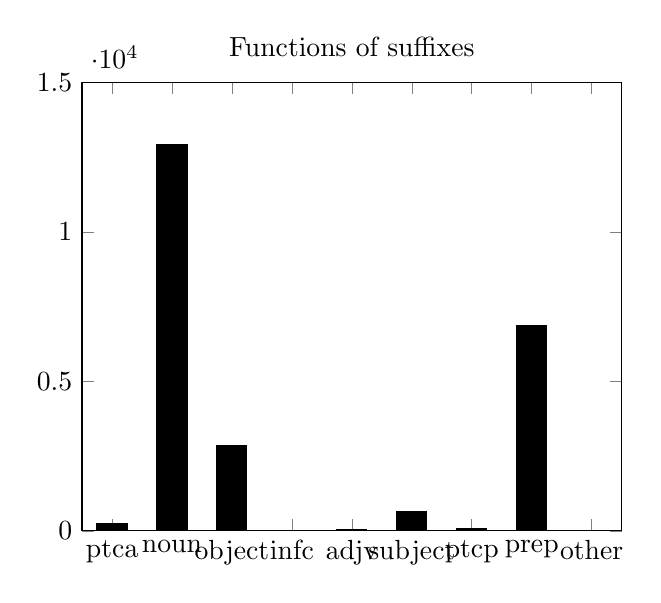
\begin{tikzpicture}[baseline]
\begin{axis}[
title = Functions of suffixes,
xmin=-0.5, xmax=8.5,
ymin=0, ymax=15000,
xtick={0,1,2,3,4,5,6,7,8},
xticklabels={ptca,noun,object,infc,adjv,subject,ptcp,prep,other},
xticklabel style = {\xticklabel},
]
\draw[draw=\bardrawcolor,fill=\barcolor] (axis cs:-0.25,0) rectangle (axis cs:0.25,246);
\draw[draw=\bardrawcolor,fill=\barcolor] (axis cs:0.75,0) rectangle (axis cs:1.25,12916);
\draw[draw=\bardrawcolor,fill=\barcolor] (axis cs:1.75,0) rectangle (axis cs:2.25,2854);
\draw[draw=\bardrawcolor,fill=\barcolor] (axis cs:2.75,0) rectangle (axis cs:3.25,6);
\draw[draw=\bardrawcolor,fill=\barcolor] (axis cs:3.75,0) rectangle (axis cs:4.25,40);
\draw[draw=\bardrawcolor,fill=\barcolor] (axis cs:4.75,0) rectangle (axis cs:5.25,646);
\draw[draw=\bardrawcolor,fill=\barcolor] (axis cs:5.75,0) rectangle (axis cs:6.25,78);
\draw[draw=\bardrawcolor,fill=\barcolor] (axis cs:6.75,0) rectangle (axis cs:7.25,6862);
\draw[draw=\bardrawcolor,fill=\barcolor] (axis cs:7.75,0) rectangle (axis cs:8.25,2);
\end{axis}
\end{tikzpicture}

